%\chapter{det-comp}


%%%%%%%%%%%%%%%%%%%%%%%%%%%%%%%%%%%%%%%%%%%%%%
%\section{Anode Plane Assemblies}

%%%%%%%%%%%%%%%%%%%%%%%%%%%%%%%%%%%%%%%%%%%%%%
%\section{Cathode Plane Assemblies}

%%%%%%%%%%%%%%%%%%%%%%%%%%%%%%%%%%%%%%%%%%%%%%
\section{Field Cage}

\subsection{Scope, Requirements and Design Parameters}
\begin{itemize}
\item Field uniformity
\item Modularity
\item Compatibility with FD design
\item Discharge behavior
\end{itemize}

\subsection{Electrical Design}

\subsubsection{Electrostatic analysis}

\subsubsection{Surge suppressor on field cage}

\subsubsection{Resister tolerance and spec}

\subsubsection{Electrical Schematic}
 

\subsection{Validation tests of roll formed FC design}

A dedicated test setup has been designed and constructed to validate the field cage concept  in purified LAr.
It consists of a field cage (Figure~\ref{fig:fc-test}), fitting into the ICARUS 50 liter cryostat (1.1 m hight, 0.6 m diameter) available at CERN, and  including:

\begin{itemize}	
\item Roll-formed metal profiles with UHMW PE caps.
\item Pultruded fiberglass I-beams form 4 mini panels.
\item HV cable feed-through (equipped with corona monitor) allowing to apply up to 150 kV on FC profiles.
\item All profiles are at same potential to simplify HV connection
\item ICARUS-like stainless steel ground planes placed  66mm away from FC profiles (~1/3 of FD bias voltage to reach
same E field)
\item Video cameras in Gas phase to monitor bubbles and sparks.
\end{itemize}

\begin{cdrfigure}[The field cage test setup]{fc-test}{The field cage test setup. 
 {\bf Left:} schematic drawings of the cage showing the main elements: metal profiles, I-beams, ground planes.
  {\bf Right:} Picture of the realized setup.}
\includegraphics[width=0.45\linewidth]{tpc_fc-test-1.png}
\includegraphics[width=0.45\linewidth]{tpc_fc-test-2.png}
\end{cdrfigure}

Two choices of material (Aluminum, Stainless Steel) for the metal profiles have been tested. In the Aluminum case, the surface finish has also been tested with scratches up to 100 um deep. 

The cage was operated both in commercial LAr and, connected to the ICARUS 50 liter recirculation system, in LAr  with purity  better that 0.1 ppb O2 equivalent. HV above 80 kV (corresponding to an electric field about 20\% higher than nominal) could be applied for several days, without recording any discharge. Two additional regimes have been studied:
\begin{itemize}	
\item  with the 50 liter vessel fully thermalized (no visible bubble formation along the detector) no sparks ever recorded up to 100 kV.
\item  HV instabilities arise in the 80-100 kV range if the LAr is not perfectly thermalized allowing bubble formation from heat sources (HV feedthrough, ground connections): few random sparks recorded, developing however around the HV cable and not between the field cage and the ground plates
\end{itemize}

All tested materials exhibited the same behaviour in the applied HV range. 

Nickel coating (up to 20 um) of aluminum profiles was also proposed  to avoid oxidation of the surface which could possibly be a source of HV instability. Its stability against  thermal gradients was positively tested. However HV tests showed no difference with respect to the uncoated version.

A specific Breakdown Test has been performed to check dielectric rigidity of the UHMW PE end caps in LAr, exposing few metal profiles equipped with PE end caps and connected the HV, to a ground plane (Figure~\ref{fig:endcap-test}).

Results demonstrated that the proposed end cap geometry and thickness can safely hold 150 kV.

\begin{cdrfigure}[Setup to test dielectric rigidity]{endcap-test}{Setup to test dielectric rigidity of the UHMW PE end caps}
\includegraphics[width=0.65\linewidth]{tpc_fc_endcap-test.png}
\end{cdrfigure}





\subsection{Ground Plane Design}
%% by A. Zani

In order to confine the electric field in the liquid argon region, it is foreseen to install a metallic plane, put to ground, between the upper field cage module and the liquid-gas interface. The design of such Ground Plane (GP) is inspired by the one from the ICARUS T600 detector, and it is meant to limit the residual electric field in the liquid below the usual 30 kV/cm. value. The design details of the planes were verified to comply with the requests on residual electric field with FEA. It is noted that a similar GP could be added in front of all the other Field Cage (FC) modules, in order to smooth the field in the LAr dead volume. However, so far it is foreseen to add an actual GP only below the bottom FC, to further smooth the field in the region where pipings for the cryostat filling are running. The distance between the cryostat walls and the end-wall field cage does not require to insert a GP, instead.

As mentioned, the GP design is inspired by the ICARUS T600 detector: in that case, 1 mm thick Stainless Steel (SS) plates, punched with $10$ mm holes, 15 mm pitch ($\sim 50\%$ transparency), could stand a potential differential of $-150$ kV over $100$ mm. In order to smooth the field, the edges of the planes were rounded to $\sim 10$ mm. The fraction of punched structure was selected to ensure light-weight even with SS, and to allow fluid circulation above the planes.

In the ProtoDUNE configuration, the GP will be put at a distance of 200 mm from the FC profile, with a structure of $6$ mm holes, $10$ mm pitch ($\sim 25\%$ transparency): the lower fraction of pierced surface is verified by simulations to maintain the field within the required values. The edges of the plates, $20$ mm high, are rounded at $5$ mm, while the holes rounding radius, at production is around $0.5$ mm. The liquid level is expected to be at 40 mm above the GP bottom, i.e. 20 mm above the edges. The radius of curvature for the holes is not a strict requirement. It depends on the punching technique, and usually is at around $0.5$ mm. The actual requirement is to have the hole curvature on the inside (of the TPC) looking out.

Two sets of pieces were initially produced in Europe:
\begin{itemize}
\item 8 pieces of dimension $198 \times 571$ mm (weight $< 1$ kg each) to be installed in the CERN field cage prototype,
\item 6 more pieces of  $525 \times 2318$ mm (weight around $8.5$ kg each), which represent full scale components for ProtoDUNE. The drawing of this second set of pieces, sent to US for test assemblies, in shown in Figure~\ref{fig:gp_panels}.
\end{itemize}

\begin{cdrfigure}[ProtoDUNE GP]{gp_panels}{Top: Techincal Drawing, by Claudio Montanari, of the Ground Plane panels for ProdoDUNE. Bottom: 3D model of one panel}
\includegraphics[width=1.0\linewidth]{tpc_fc_gp525x2318piece.png}
\end{cdrfigure}


The choice of electropolished Stainless Steel \textit{AISI 304 L} over Aluminum derives from the experience of the ICARUS detector, moreover:
\begin{itemize}
\item SS and G10 have very similar dilatation coefficients, while Aluminum does not. Choosing SS ensures that all the $GP\,+\,G10$ structure contracts consistently, without too large stresses at the connections; 
\item SS is more ductile than Aluminum, which makes \textit{easier} to machine the corners of the pieces. Note that anyway some imperfections are present even in the SS case, and not all corners will be perfectly identical. 
\item Though Aluminum would guarantee a factor 3 lighter GP, the overall weight of the SS pieces remains contained (order of 550 kg).
\end{itemize}

\subsection{Field Cage prototype at CERN}
The main description of the Field Cage Prototype built at CERN, and the tests performed on it, is provided in section ... .In here simply the details concerning the GP are reminded. The smaller pieces of GP were installed on the field cage prototype at CERN, to test the configuration. As described elsewhere, the actual distance between the field cage profiles and the GP in this prototype is of 60 mm, therefore a voltage of 60 kV minimum must be attained to verify the ProtoDUNE field configuration. (Figure ~\ref{fig:fc_prot}) During multiple tests in LAr, both with open-air dewars and in a clean liquid configuration, the structure always stood the 60 kV voltage, and it was in general possible to reach the value of 80-100 kV, after which discharges would start. However discharges were always localized on the HV cables, not involving the GP-FC structure.

\begin{cdrfigure}[CERN Prototype]{fc_prot}{Details of the Field Cage Prototype at CERN, showing the installed GP panels.}
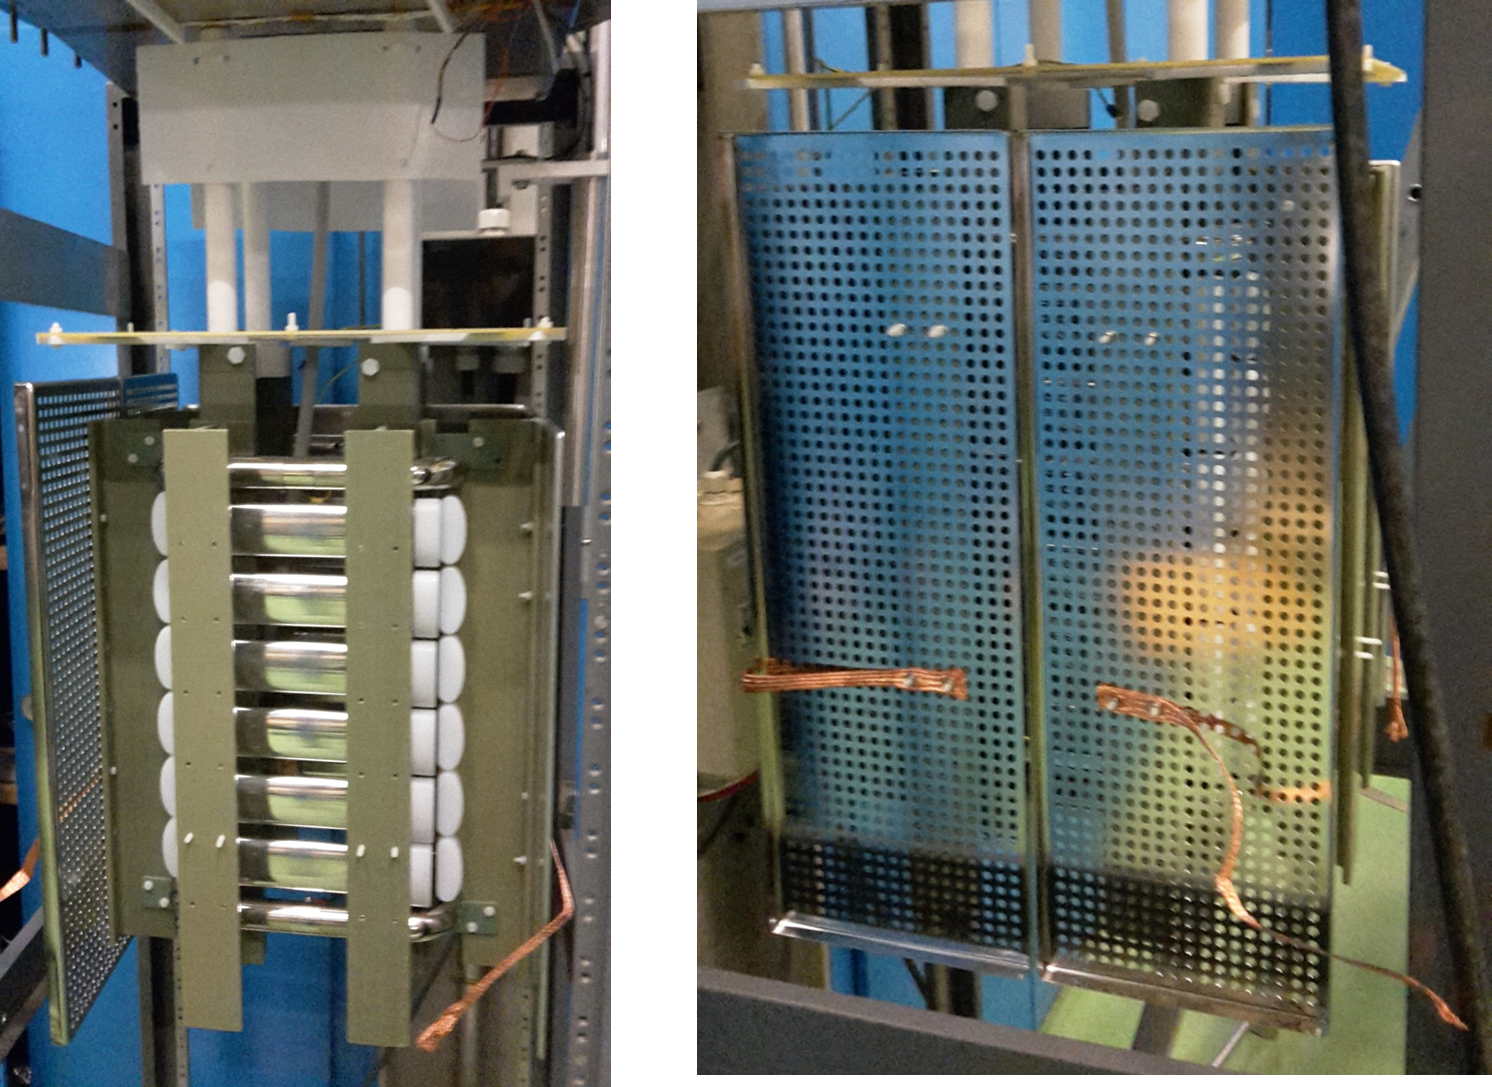
\includegraphics[width=0.8\linewidth]{tpc_fc_prototype.png}
\end{cdrfigure}

\subsection{Field Cage and Ground Plane in ProtoDUNE}

Latest design of the FC+GP modules for ProtoDUNE was produced by Rahul Sharma: it is described and shown in section ... . Here a 3D model of one fully assembled module is shown for understanding in Figure ~\ref{fig:fc_full}.

\begin{cdrfigure}[CERN Prototype]{fc_full}{3D model of one fully assembled FC+GP module, for the top of the field cage. }
\includegraphics[width=0.8\linewidth]{tpc_topFC.png}
\end{cdrfigure}

One module will be made of 6 pieces, put next to each other along the 2318 mm direction: this dimension is made to match the APA and FC module widths. The planes are connected to the FC beam with further G10 pieces that are used also to connect two neighboring GP panels.

The electrical continuity between consecutive panels can be performed with metallic screws (with holes on the planes edges) or with looser connections, like copper strips, that better adapt to the shrinking of the structure during cool-down. Copper strips were successfully employed on the CERN FC prototype.
As for most detector systems, the GP should be referenced to the detector ground, set at cryostat top.

The GP modules will be installed on the corresponding FC modules in the clean room outside the cryostat, to facilitate the connections. The description of how the top/bottom FC modules are assembled and connected to the CPA before insertion in the cryostat is provided in section ... .

Further GP panels need to be attached to the top FC module:
\begin{itemize}
\item smaller panels will have to be connected on the modules on one side of the CPA so that, once in position, they should cover the CPA frame. Their dimension is still to be defined, depending on the final design of the CPA hanging scheme. Such pieces should also be connected to the modules covering the opposite drift region, when in final position;
\item a further set of small panels should be installed on the outer modules of the FC, to extend the GP over the vertical FC walls, to further constrain the electric field in these regions. A FEA (Figure ~\ref{fig:fea_overhang}) shows that the optimized overhang distance is 20 cm, provided LAr is at 40 mm above the GP bottom. The maximal residual field in this configuration is of the order of 13 kV/cm, with less than 1 kV/cm field in the gas phase.
\end{itemize}

\begin{cdrfigure}[FEA overhang]{fea_overhang}{2D FEA showing the field profile in liquid with a 200 mm overhang, gas-liquid interface 40 mm above the GP bottom. Highest field in the liquid phase is of the order of 13 kV/cm.}
\includegraphics[width=0.7\linewidth]{tpc_fc_gp_overhang.png}
\end{cdrfigure}








\subsection{Designs of the Field Cage Modules}

\subsubsection{Top and bottom modules}

\subsubsection{End wall modules}



\subsection{Interfaces to Other TPC Components}

\subsubsection{Field cage to CPA}

\subsubsection{Field cage to APA}

\subsubsection{Field cage to beam plug}

\subsubsection{Field cage to calibration lasers}



\subsection{Assembly Sequence and QC Procedures}


\subsection{Installation Sequence}
\fixme{Do we have an installation section?}



 


